\chapter{Scheduling}
\newpage

\section{Scheduler, Processi e Thread}
\subsection{Introduzione}
Un sistema operativo è un gestore di risorse come: processore, memoria principale e secondaria, dispositivi. Per svolgere i suoi compiti, un sistema operativo ha bisogno di strutture dati per mantenere informazioni sulle risorse gestite.
Queste strutture dati comprendono: tabelle di memoria, tabelle di I/O, tabelle del file system e tabelle dei processi.

\subsubsection{Tabelle per la gestione della memoria}
Allocazione memoria per il sistema operativo, 
allocazione memoria principale e secondaria per i processi,
informazioni per i meccanismi di protezione.

\subsubsection{Tabelle per la gestione dell'I/O}
Informazioni sullo stato di assegnazione dei dispositivi utilizzati dalla macchina, gestione di code di richieste.

\subsubsection{Tabelle per la gestione del file system}
Elenco dei dispositivi utilizzati per mantenere il file system, elenco dei file aperti e loro stato.

\begin{figure}[h]
    \centering
    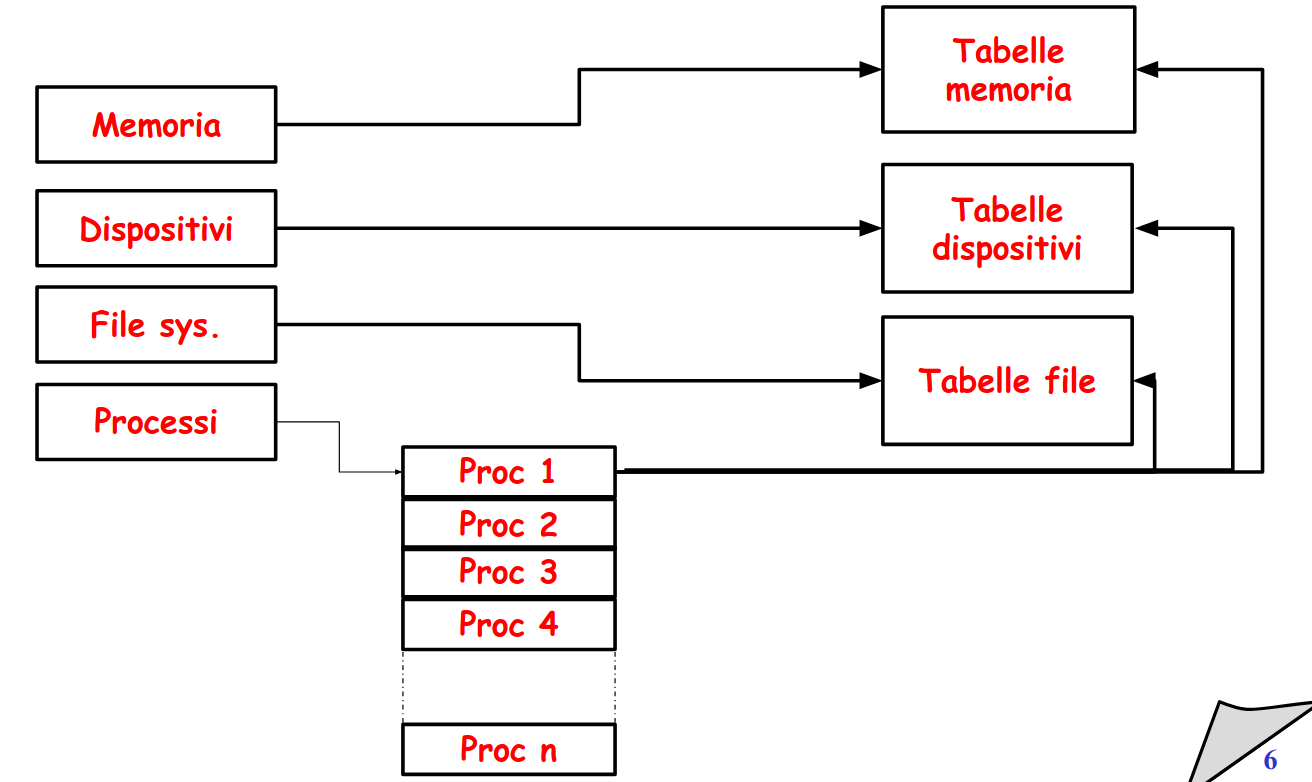
\includegraphics[width=0.7\linewidth]{Images/Screenshot 2024-12-18 at 15-07-44 so-02.1-scheduling - so-02.1-scheduling.pdf.png}
    \caption{Tabelle per la gestione}
\end{figure}

\subsection{Descrittori dei processi}
\paragraph{Qual é la manifestazione fisica di un processo?}

\begin{enumerate}
    \item il codice da eseguire (segmento codice)
    \item i dati su cui operare (segmenti dati)
    \item uno stack di lavoro per la gestione di chiamate di funzione, passaggio di
parametri e variabili locali
    \item un insieme di attributi contenenti tutte le informazioni necessarie per la gestione del processo stesso

\end{enumerate}

Questo insieme di attributi prende il nome di descrittore del processo (process control block, PCB).

\begin{figure} [h]
    \centering
    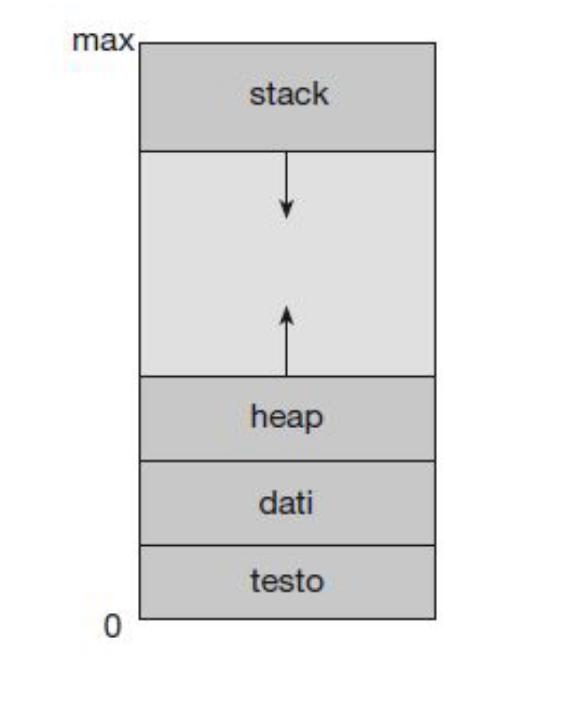
\includegraphics[width=0.3\linewidth]{Images/Screenshot 2024-12-18 at 18-22-19 so-02.1-scheduling - so-02.1-scheduling.pdf.png}
    \caption{Processo in memoria}
\end{figure}
\newpage
\paragraph{Tabella per la gestione dei processi:} contiene i descrittori dei processi, ogni processo ha un descrittore associato.
E' possibile suddividere le informazioni contenute nel descrittore in tre aree:
\begin{itemize}
    \item informazioni di identificazione di processo
    \item informazioni di stato del processo
    \item informazioni di controllo del processo
\end{itemize}

\subsubsection{Informazioni di identificazione di un processo}
L'identificatore di processo (process id, o pid), può essere semplicemente un indice all'interno di una tabella di processi.
Può essere un numero progressivo; in caso, è necessario
un mapping tra pid e posizione del relativo descrittore, molte altre tabelle del s.o. utilizzano il process id per identificare un elemento della tabella dei processi.

Possono essere identificatori di altri processi logicamente collegati al processo. \textit{Ad esempio, pid del processo padre}

Id dell'utente che ha richiesto l'esecuzione del processo

\subsubsection{Informazioni di stato del processo}
Come registri generali del processore o registri speciali, come il program counter e i registri di stato.

\subsubsection{Informazioni di controllo del processo}
\textbf{Informazioni di scheduling:} stato del processo (in esecuzione, pronto, in attesa), informazioni particolari necessarie dal particolare algoritmo di scheduling utilizzato, identificatore dell'evento per cui il processo è in attesa.
\newline
\textbf{Informazioni di gestione della memoria:} valori dei registri base e limite dei segmenti utilizzati, puntatori alle tabelle delle pagine, etc.
\newline
\textbf{Informazioni di accounting:} tempo di esecuzione del processo, tempo trascorso dall'attivazione di un processo.
\newline
\textbf{Informazioni relative alle risorse:} risorse controllate dal processo, come file aperti, device allocati al processo.
\newline
\textbf{Informazioni per interprocess communication (IPC):} stato di segnali, semafori, etc.

\subsection{Scheduler}
Lo scheduler è la componente più importante del kernel, gestisce l'avvicendamento dei processi decidendo quale processo deve essere in esecuzione ad ogni istante, interviene quando viene richiesta un'operazione di I/O e quando un'operazione di I/O termina, ma anche periodicamente.

\begin{figure} [h]
    \centering
    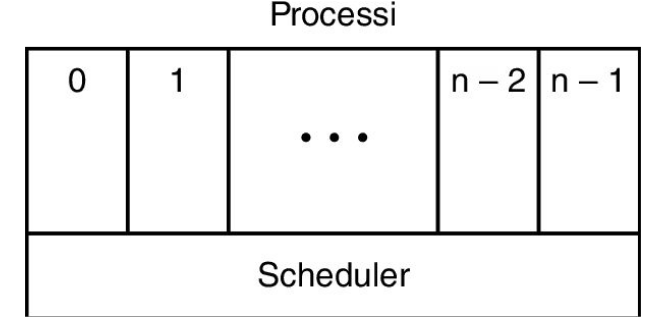
\includegraphics[width=0.35\linewidth]{Images/Screenshot 2024-12-18 at 18-47-56 so-02.1-scheduling - so-02.1-scheduling.pdf.png}
\end{figure}
\textbf{Schedule:} è la sequenza temporale di assegnazioni delle risorse da gestire ai richiedenti.

\textbf{Scheduling:} è l'azione di calcolare uno schedule.

\textbf{Scheduler:} è la componente software che calcola lo schedule.

\subsection{Mode switching e Context switching}
Tutte le volte che avviene un interrupt (software o hardware) il
processore è soggetto ad un \textbf{mode switching} (modalità utente → modalità supervisore)
Durante la gestione dell'interrupt vengono intraprese le opportune azioni per gestire l'evento. Viene chiamato lo scheduler: se lo scheduler decide di eseguire un altro processo, il sistema è soggetto ad un \textbf{context switching}.

Durante un context switching, lo stato del processo attuale viene salvato nel PCB corrispondente mentre lo stato del processo selezionato per l'esecuzione viene caricato dal PCB
nel processore.
\begin{figure} [h]
    \centering
    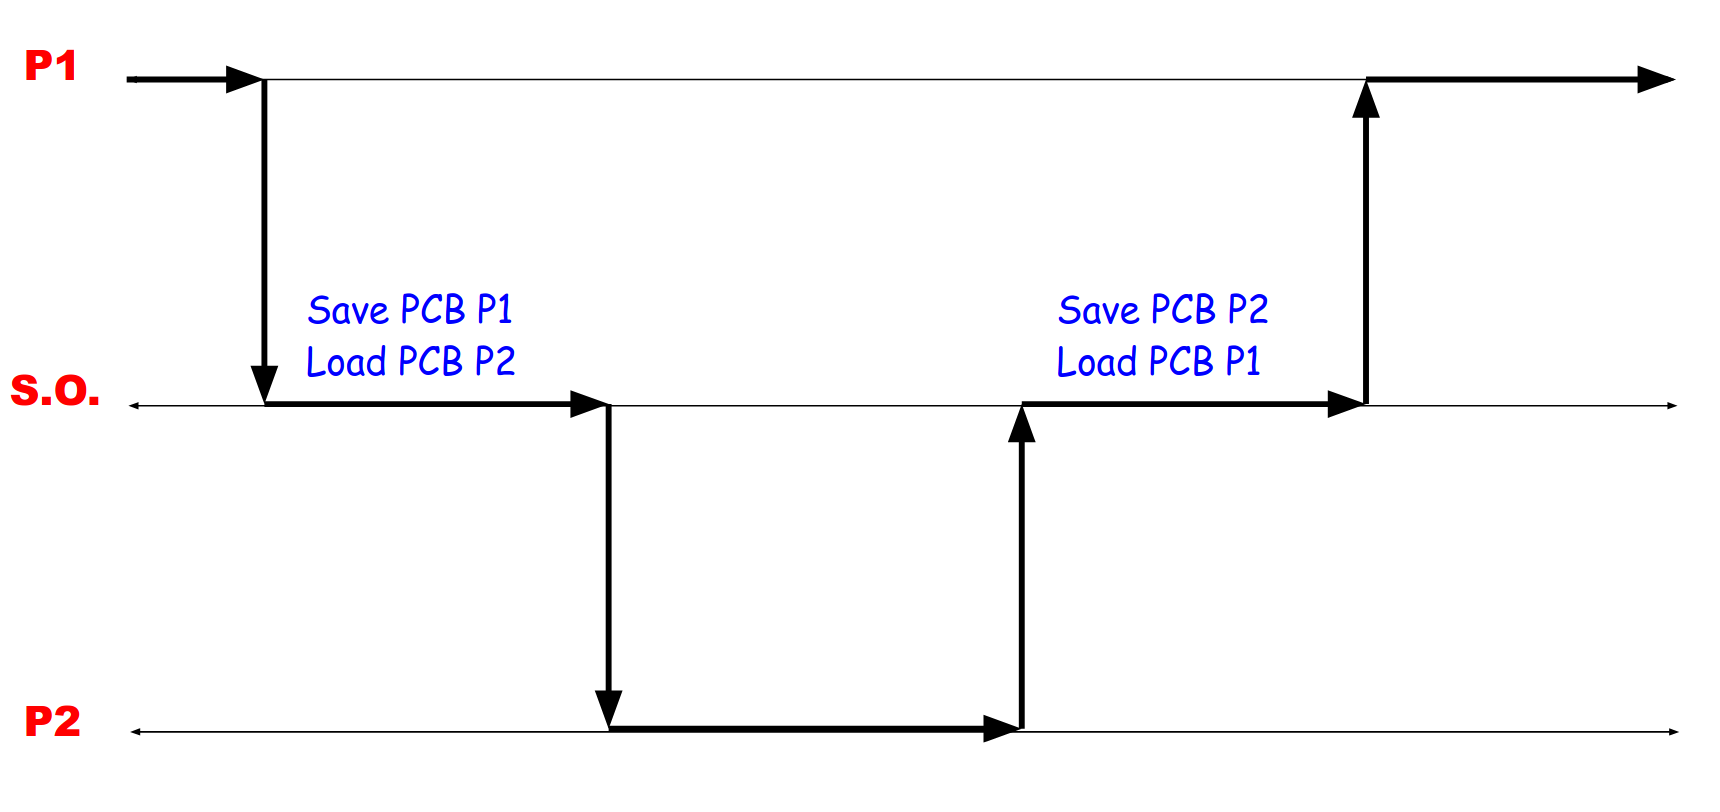
\includegraphics[width=0.6\linewidth]{Images/Screenshot 2024-12-18 at 18-58-00 so-02.1-scheduling - so-02.1-scheduling.pdf.png}
    \caption{Funzionamento del context switch}
\end{figure}




\subsection{Processi e Thread}

\subsubsection{Vita di un processo}
Gli stati di un processo possono essere:
\newline

\textbf{Running:} il processo è in esecuzione.

\textbf{Waiting:} il processo è in attesa di qualche evento esterno (e.g., completamento.
operazione di I/O); non può essere eseguito.

\textbf{Ready:} il processo può essere eseguito, ma attualmente il processore è impegnato in altre attività.

\begin{figure} [h]
    \centering
    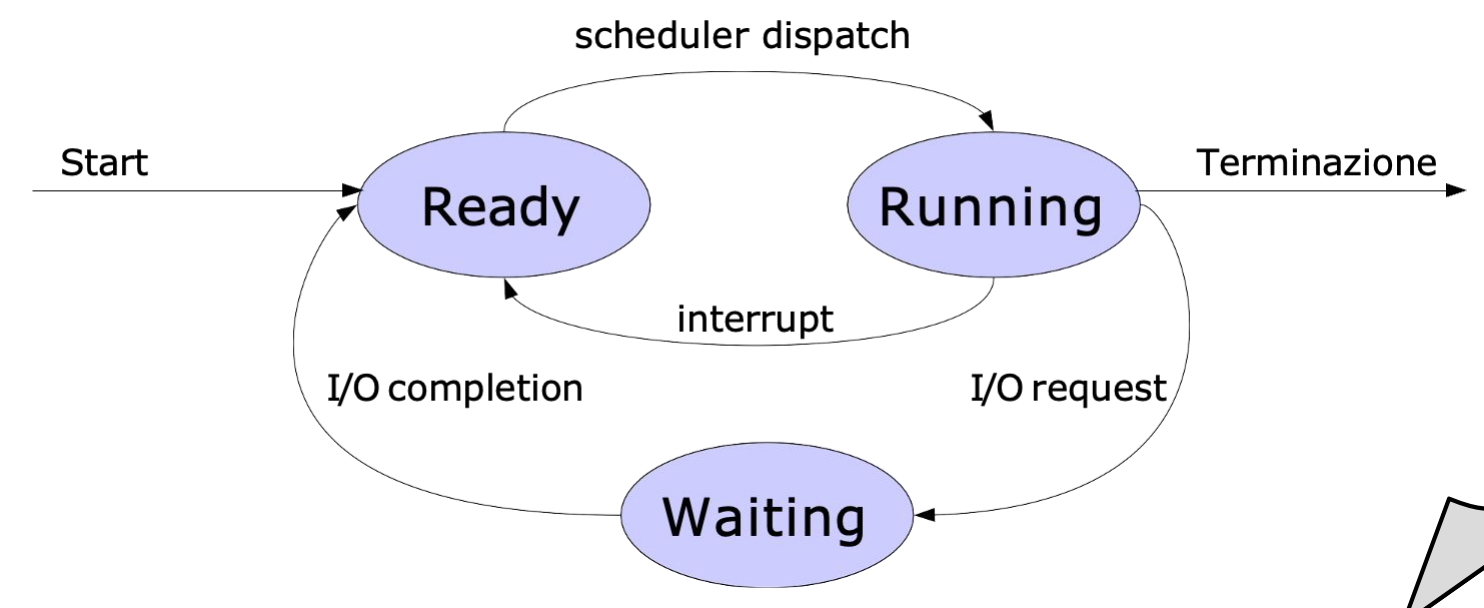
\includegraphics[width=0.6\linewidth]{Images/Screenshot 2024-12-23 at 12-34-55 so-02.1-scheduling - so-02.1-scheduling.pdf.png}
    \caption{Stati dei processi}
\end{figure}

Tutte le volte che un processo entra nel sistema, viene posto in una delle code gestite dallo scheduler.

\begin{figure} [h]
    \centering
    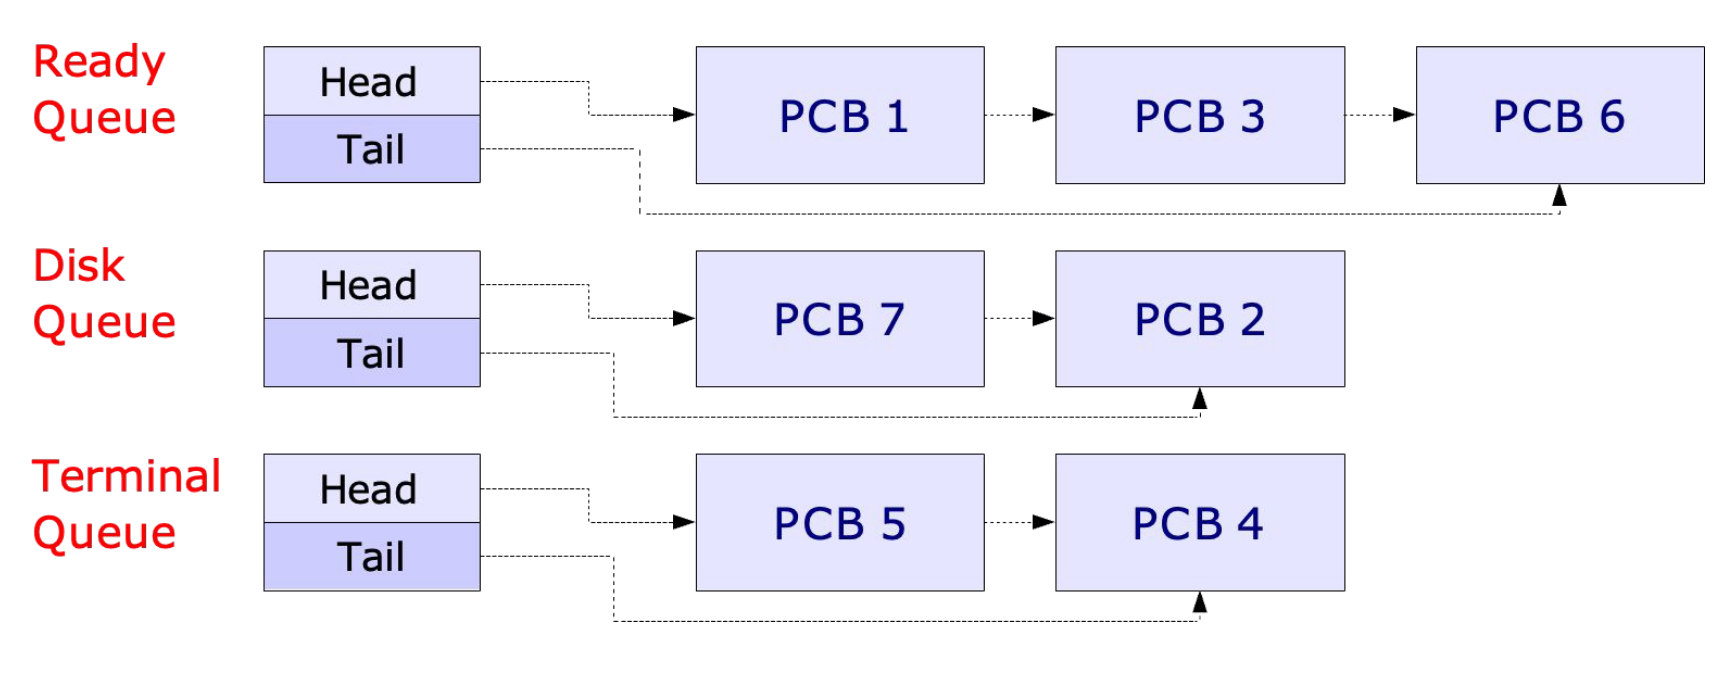
\includegraphics[width=0.6\linewidth]{Images/Screenshot 2024-12-23 at 12-37-44 so-02.1-scheduling - so-02.1-scheduling.pdf.png}
    \caption{Le code gestite dallo scheduler}
\end{figure}

\subsubsection{Gerarchia di processi}
Nella maggior parte dei sistemi operativi i processi sono organizzati in forma gerarchica.

Quando un processo crea un nuovo processo, il processo creante viene
detto padre e il creato figlio
si viene così a creare un albero di processi.

Le motivazioni sono la semplificazione del procedimento di creazione di processi, non occorre specificare esplicitamente tutti i parametri e le caratteristiche e ciò che non viene specificato, viene ereditato dal padre.

\begin{figure}[h]
    \centering
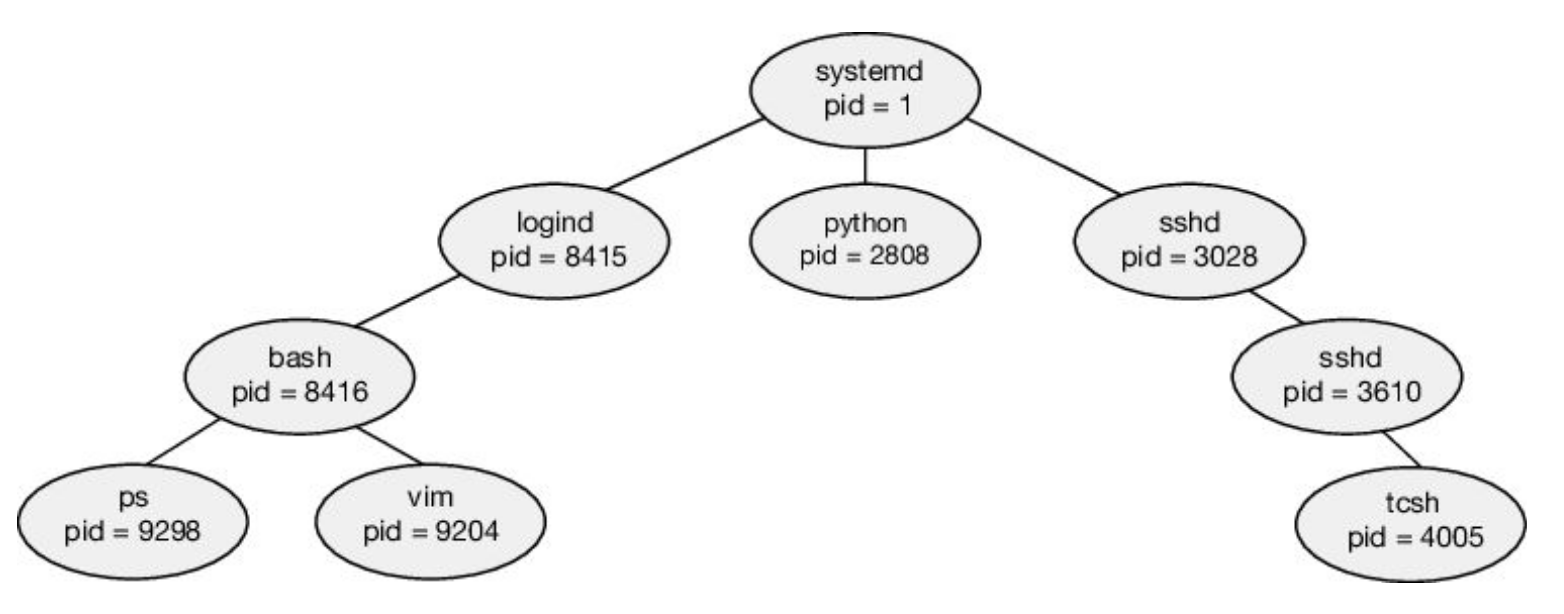
\includegraphics[width=0.6\linewidth]{Images/Screenshot 2024-12-23 at 12-42-11 so-02.1-scheduling - so-02.1-scheduling.pdf.png}
    \caption{Albero dei processi di un sistema Linux}
\end{figure}

\subsubsection{Threads}
\paragraph{}
La nozione di processo discussa in precedenza assume che ogni
processo abbia una singola “linea di controllo”. Per ogni processo, viene eseguite una singola sequenza di istruzioni, un singolo processo non può eseguire due differenti attività
contemporaneamente.

\textit{Esempi: scaricamento di due differenti pagine in un web browser, inserimento di nuovo testo in un wordprocessor mentre viene eseguito il correttore ortografico}

\paragraph{}
Tutti i sistemi operativi moderni supportano l’esistenza di processi \textbf{multithreaded}. In un processo multithreaded esistono molte “linee di controllo”, ognuna
delle quali può eseguire un diverso insieme di istruzioni.

\textit{Esempi: Associando un thread ad ogni finestra aperta in un web browser, è possibile scaricare i dati in modo indipendente.
}

\paragraph{Cos'è un thread?}
Un thread è l’unità base di utilizzazione della CPU.
Ogni thread possiede la propria copia dello stato del processore, il proprio program counter e uno stack separato.
I thread appartenenti allo stesso processo condividono: codice, dati e risorse di I/O.

\begin{figure} [h]
    \centering
    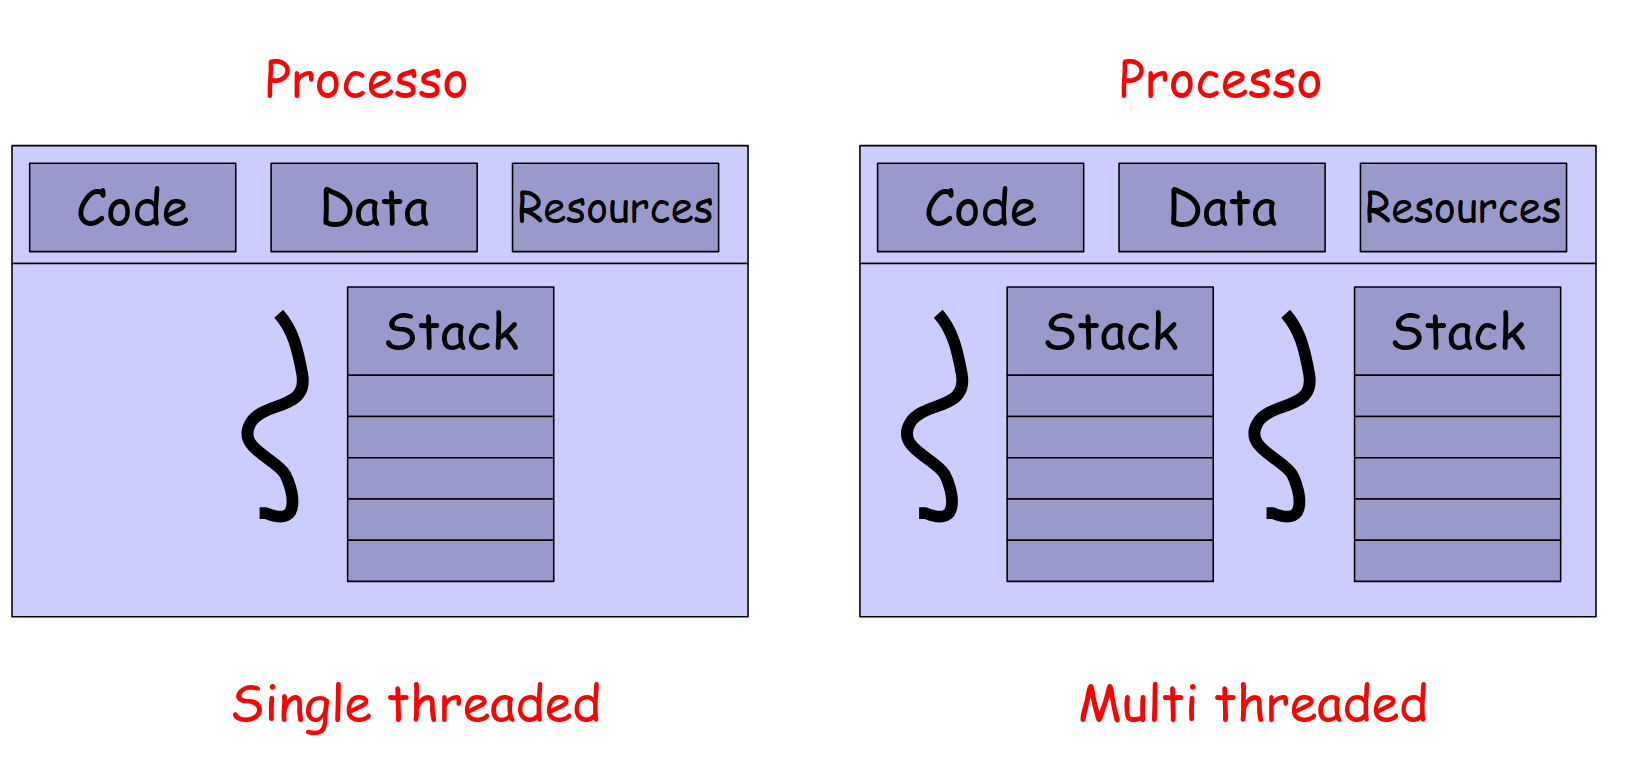
\includegraphics[width=0.6\linewidth]{Images/Screenshot 2024-12-23 at 12-51-01 so-02.1-scheduling - so-02.1-scheduling.pdf.png}
    \caption{Singlethreaded e multithreaded}
\end{figure}

\paragraph{Benefici dei thread}
La condivisione di risorse: i thread condividono lo spazio di memoria e le risorse allocate degli altri thread dello stesso processo. Condividere informazioni tra thread logicamente correlati rende più semplice l’implementazione di certe applicazioni.

\textit{Esempio: web browser: condivisione dei parametri di configurazione fra i vari thread.}
\newline

Economia: allocare memoria e risorse per creare nuovi processi è costoso, fare context switching fra diversi processi non è ottimale. 
Mentre gestire i thread è in generale più economico, creare thread all’interno di un processo permette di fare context switching fra thread che è meno costoso.

\textit{Esempio: creare un thread in Solaris richiede 1/30 del tempo richiesto per creare un nuovo processo.}

\textbf{Thread = processi "lightweight"}
Utilizzare i thread al posto dei processi rende l’implementazione più efficiente. In ogni caso, abbiamo bisogno di processi distinti per applicazioni differenti.

\subsection{Multithreading}

Un sistema operativo può implementare i thread in due modi:
\begin{itemize}
    \item User thread
    \item Kernel thread
\end{itemize}

\subsubsection{User thread}
Gli user thread vengono supportati sopra il kernel e vengono
implementati da una \textbf{thread library} a livello utente. La thread library fornisce supporto per la creazione, lo scheduling e la gestione dei thread senza alcun intervento del kernel.

\textbf{Vantaggi:} l’implementazione risultante è molto efficiente.
\newline

\textbf{Svantaggi:} Se il kernel è single-threaded, qualsiasi user thread che effettua una chiamata di sistema bloccante (che si pone in attesa di I/O) causa il blocco dell’intero processo.

\subsubsection{Kernel thread}
I kernel thread vengono supportati direttamente dal sistema
operativo. La creazione, lo scheduling e la gestione dei thread sono implementati a livello kernel.

\textbf{Vantaggi:} poichè è il kernel a gestire lo scheduling dei thread, se un thread esegue una operazione di I/O, il kernel può selezionare un altro thread in attesa di essere eseguito.
\newline

\textbf{Svantaggi:} l’implementazione risultante è più lenta, perché richiede un passaggio da
livello utente a livello supervisore

\subsubsection{Modelli di multithreading}
Molti sistemi supportano sia kernel thread che user thread.
Si vengono così a creare tre differenti modelli di multithreading:

\begin{itemize}
    \item Many-to-One
    \item One-to-One
    \item Many-to-Many
\end{itemize}

\paragraph{Many-to-One}
Un certo numero di user thread vengono mappati su un solo
kernel thread. Modello generalmente adottato da s.o. che non supportano kernel thread multipli.

\begin{figure} [h]
    \centering
    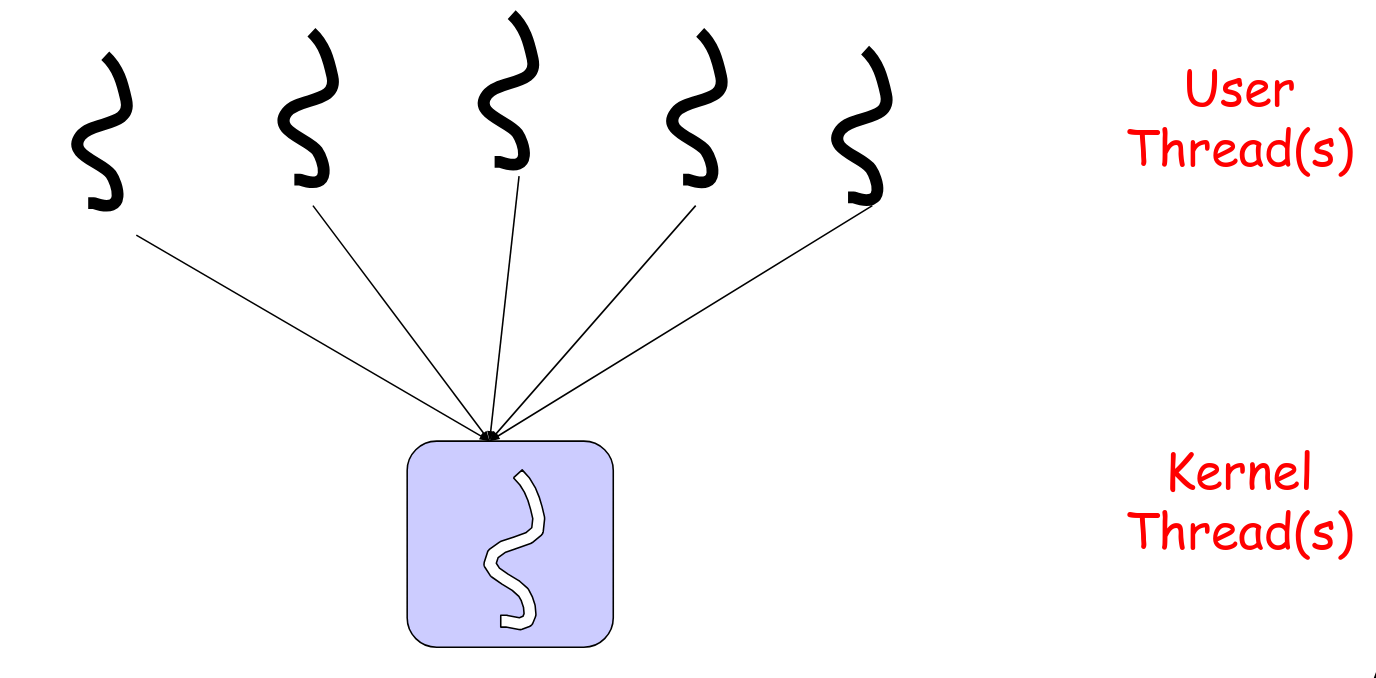
\includegraphics[width=0.5\linewidth]{Images/Screenshot 2024-12-23 at 13-14-46 so-02.1-scheduling - so-02.1-scheduling.pdf.png}
\end{figure}

\paragraph{One-to-One}
Ogni user thread viene mappato su un kernel thread. Può creare problemi di scalabilità per il kernel.

\begin{figure} [h]
    \centering
    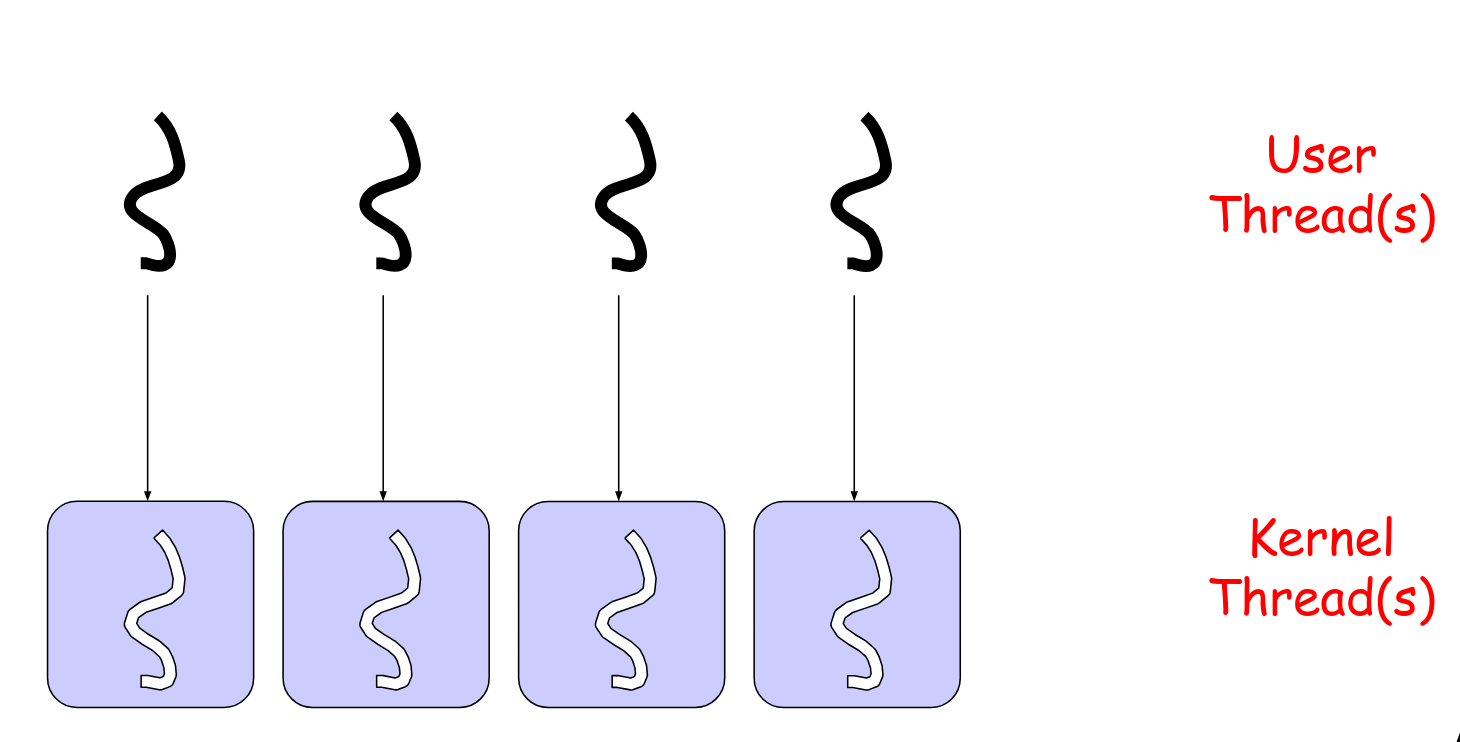
\includegraphics[width=0.5\linewidth]{Images/Screenshot 2024-12-23 at 13-16-34 so-02.1-scheduling - so-02.1-scheduling.pdf.png}
\end{figure}
\newpage
\paragraph{Many-to-Many}
Riassume i benefici di entrambe le architetture. Supportato da Solaris, IRIX, Digital Unix.

\begin{figure} [h]
    \centering
    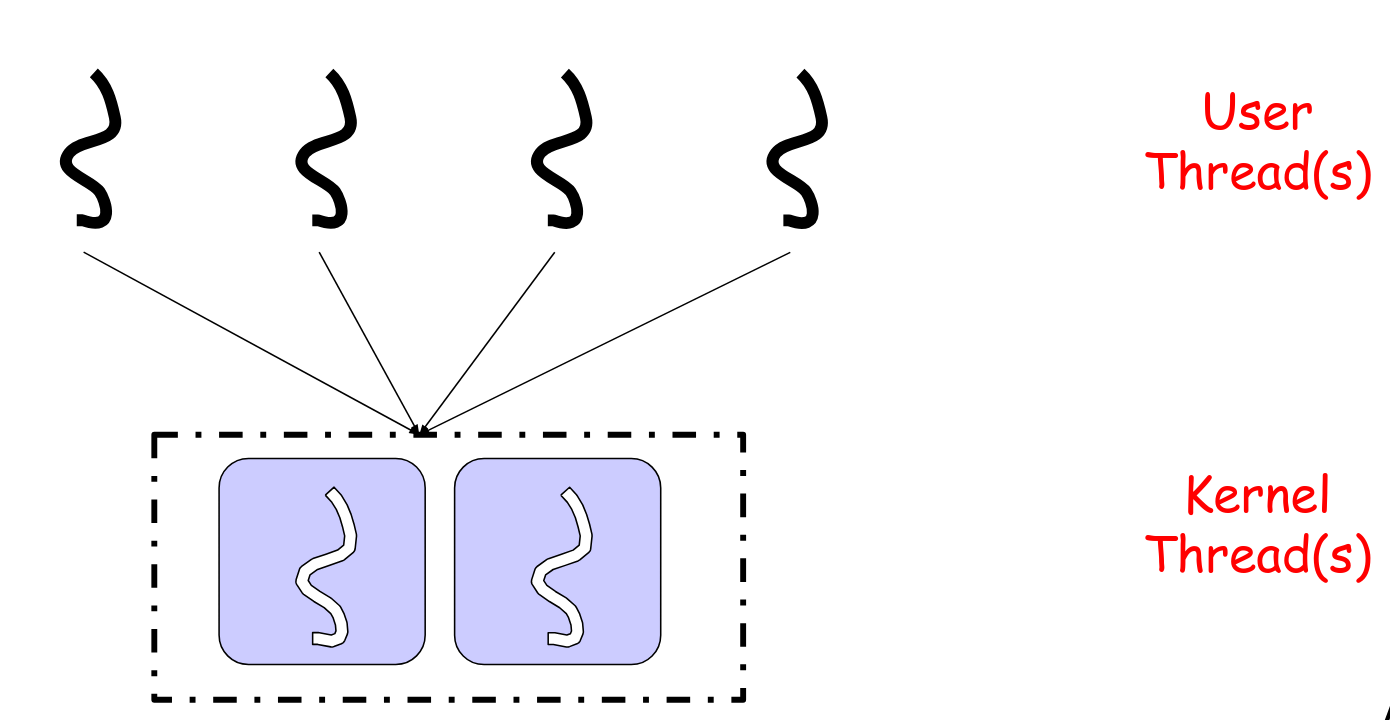
\includegraphics[width=0.5\linewidth]{Images/Screenshot 2024-12-23 at 13-17-03 so-02.1-scheduling - so-02.1-scheduling.pdf.png}
\end{figure}

\section{Schedule}

\subsection{Rappresentazione degli schedule}
Per rappresentare uno schedule si usano i diagrammi di Gantt
\begin{figure} [h]
    \centering
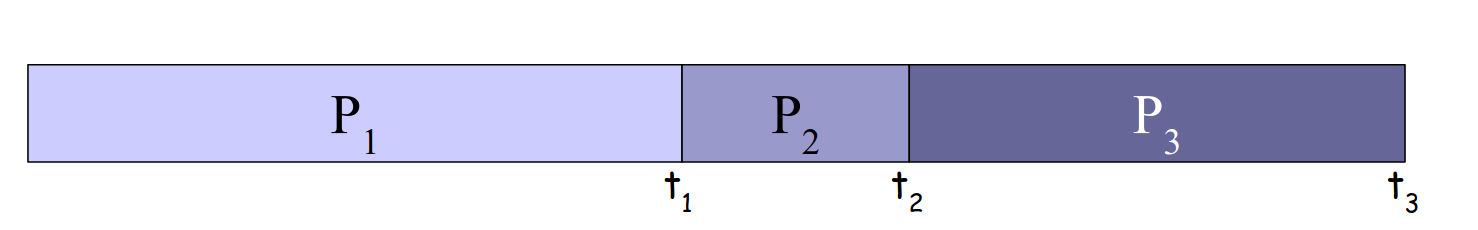
\includegraphics[width=0.5\linewidth]{Images/Screenshot 2024-12-23 at 13-32-35 so-02.1-scheduling - so-02.1-scheduling.pdf.png}
    \caption{In questo esempio, la risorsa (es. CPU) viene utilizzata dal processo $P_1$ dal tempo 0 a $t_1$, viene quindi assegnata a $P_2$ fino al tempo $t_2$ e quindi a $P_3$ fino al tempo $t_3$.}
\end{figure}
\newline

Nel caso si debba rappresentare lo schedule di più risorse (\textit{e.g., un sistema multiprocessore)} il diagramma di Gantt risulta composto da più righe parallele.

\begin{figure} [h]
    \centering
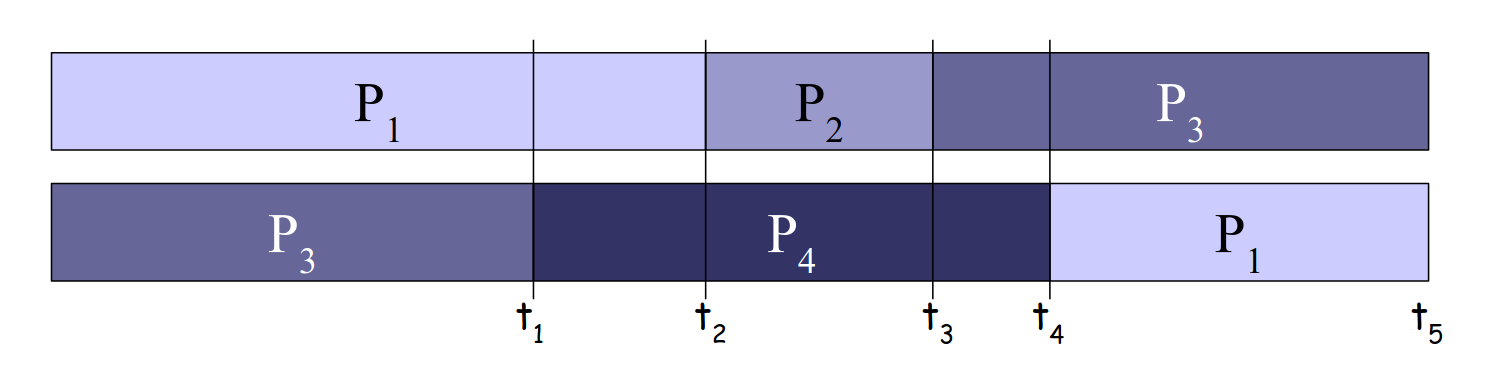
\includegraphics[width=0.5\linewidth]{Images/Screenshot 2024-12-23 at 13-37-03 so-02.1-scheduling - so-02.1-scheduling.pdf.png}
    \caption{Diagramma di Gantt multi-risorsa}
\end{figure}

\subsubsection{Tipi di scheduler}
Eventi che possono causare un context switch:
\begin{enumerate}
    \item quando un processo passa da stato running a stato waiting(system call bloccante, operazione di I/O).
    \item quando un processo passa dallo stato running allo stato ready (a causa di un interrupt).
    \item quando un processo passa dallo stato waiting allo stato ready.
    \item quando un processo termina.
\end{enumerate}

\textit{(Nota: nelle condizioni 1 e 4, l'unica scelta possibile è quella di selezionare un altro processo per l'esecuzione. Nelle condizioni 2 e 3, è possibile continuare ad eseguire il processo corrente)}
\newline

Uno scheduler si dice \textbf{non-preemptive} (o cooperativo) se i context switch avvengono solo nelle condizioni 1 e 4. In altre parole: il controllo della risorsa viene trasferito solo se l'assegnatario attuale lo cede volontariamente.
Vantaggi: non richiede alcuni meccanismi hardware come ad esempio timer programmabili.

Uno scheduler si dice \textbf{preemptive} (tutti gli scheduler moderni) se i context switch possono avvenire in ogni condizione. In altre parole: è possibile che il controllo della risorsa venga tolto all'assegnatario attuale a causa di un evento. 
Vantaggi: permette di utilizzare al meglio le risorse.
\newpage
\subsubsection{Criteri di scelta di uno scheduler}
\begin{itemize}
    \item \textbf{Utilizzo della risorsa (CPU):} lq percentuale di tempo in cui la CPU è occupata ad eseguire processi deve essere massimizzato.
    \item \textbf{Throughput:} numero di processi completati per unità di tempo. Dipende dalla lunghezza dei processi, deve essere massimizzato.
    \item \textbf{Tempo di turnaround:} tempo che intercorre dalla sottomissione di un processo alla sua terminazione, deve essere minimizzato.
    \item \textbf{Tempo di attesa:} il tempo trascorso da un processo nella coda ready, deve essere minimizzato.
    \item \textbf{Tempo di risposta:} il tempo che intercorre fra la sottomissione di un processo e il tempo di prima risposta. Particolarmente significativo nei programmi interattivi, deve essere minimizzato.
\end{itemize}

\subsubsection{Caratteristiche dei processi}
Durante l'esecuzione di un processo si alternano periodi di attività svolte dalla CPU (\textbf{CPU burst}) e periodi di attività di I/O (\textbf{I/O burst}).

I processi caratterizzati da CPU burst molto
lunghi si dicono \textbf{CPU bound}, mentre quelli caratterizzati da I/O burst molto lunghi si dicono \textbf{I/O bound}.

\begin{figure} [h]
    \centering
    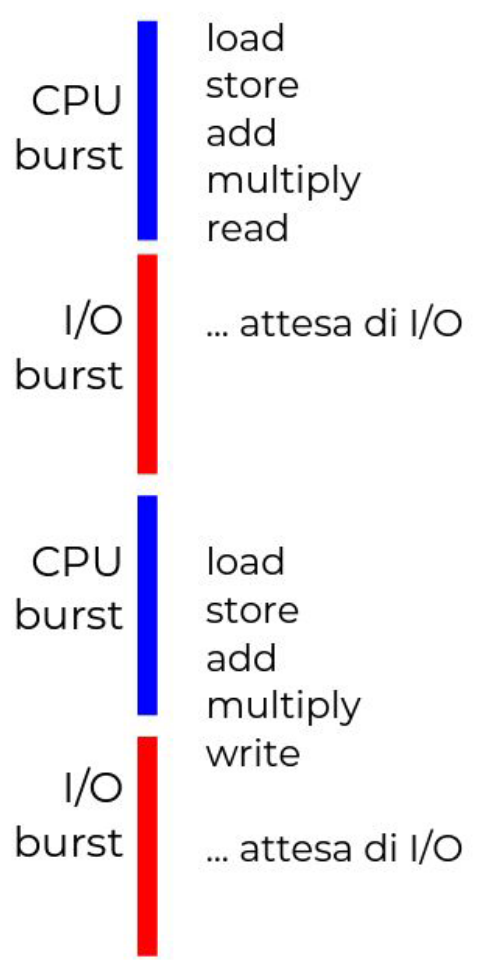
\includegraphics[width=0.2\linewidth]{Images/Screenshot 2024-12-23 at 14-20-04 so-02.1-scheduling - so-02.1-scheduling.pdf.png}
\end{figure}

\section{Algoritmi di scheduling}
Gli algoritmi di scheduling che vedremo sono:
\begin{itemize}
    \item First Come, First Served
    \item Shortest-Job First
    \begin{itemize}
        \item Shortest-Next-CPU-Burst First
        \item Shortest-Remaining-Time-First
    \end{itemize}
    \item Round-Robin
    \item Scheduling a priorità
    \item Scheduling a classi di priorità
    \item Scheduling multilivello
\end{itemize}

\subsection{First Come, First Served (FCFS)}
\paragraph{Algoritmo:} il processo che arriva per primo, viene servito per primo, politica senza preemption.

Supponiamo di avere: un processo CPU bound, un certo numero di processi I/O bound. 
I processi I/O bound si "mettono in coda" dietro al processo CPU bound, e in alcuni casi la ready queue si puo svuotare (convoy effect).

\begin{figure} [h]
    \centering
    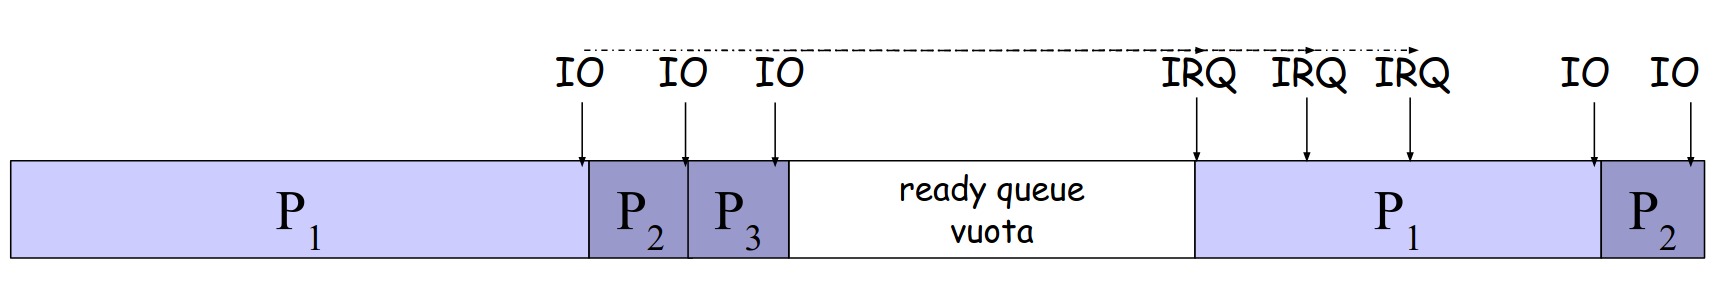
\includegraphics[width=0.5\linewidth]{Images/Screenshot 2024-12-23 at 14-30-35 so-02.1-scheduling - so-02.1-scheduling.pdf.png}
\end{figure}

\paragraph{Implementazione:} semplice, tramite una coda (politica FIFO)
\paragraph{Problemi:} elevati tempi medi di attesa e di turnaround, processi CPU bound ritardano i processi I/O bound.

\textit{Esempio:}
\begin{figure} [h]
    \centering
    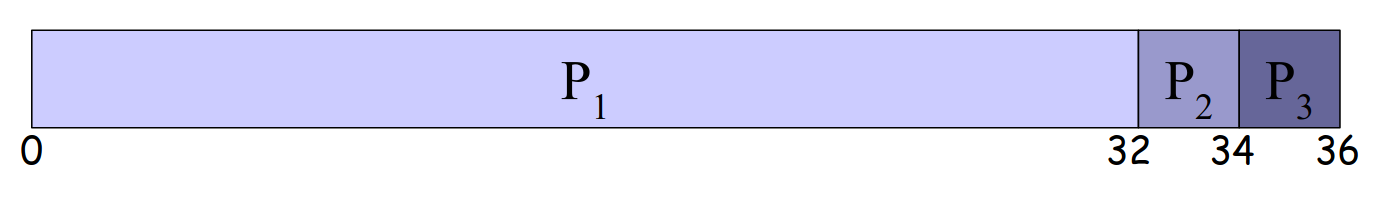
\includegraphics[width=0.5\linewidth]{Images/Screenshot 2024-12-23 at 14-25-16 so-02.1-scheduling - so-02.1-scheduling.pdf.png}
    \caption{Ordine di arrivo: $P_1$, $P_2$, $P_3$
\newline
Lunghezza dei CPU-burst in ms: 32, 2, 2
\newline
Tempo medio di turnaround: (32+34+36)/3 = 34 ms
\newline
Tempo medio di attesa: (0+32+34)/3 = 22 ms}
\end{figure}

\subsection{Shortest Job First (SJF)}
\paragraph{Algoritmo:} la CPU viene assegnata al processo ready che ha la minima durata del CPU burst successivo, politica senza preemption.

\paragraph{Problemi:} è ottimale rispetto al tempo di attesa, in quanto è possibile dimostrare che produce il minor tempo di attesa possibile, ma è impossibile da implementare in pratica! E' possibile solo fornire delle approssimazioni.

Negli scheduler long-term possiamo chiedere a chi sottomette un job di predire la durata del job.
Negli scheduler short-term non possiamo conoscere la lunghezza del prossimo CPU burst ma conosciamo la lunghezza di quelli precedenti.

\textit{Esempio:}
\begin{figure} [h]
    \centering
    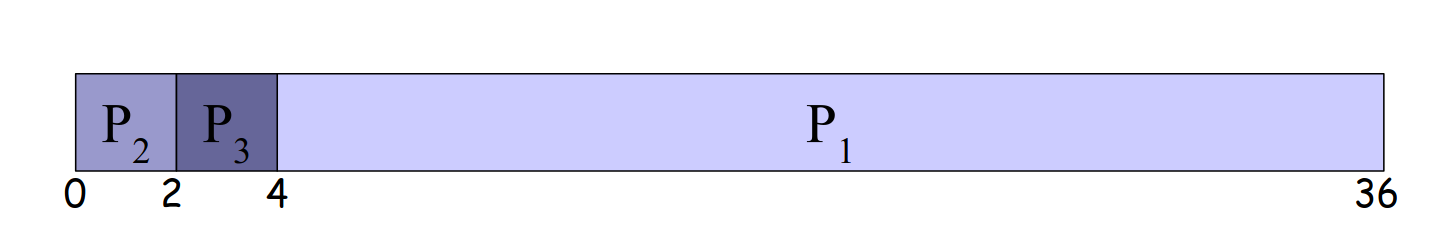
\includegraphics[width=0.5\linewidth]{Images/Screenshot 2024-12-23 at 14-33-56 so-02.1-scheduling - so-02.1-scheduling.pdf.png}
    \caption{Tempo medio di turnaround: (0+2+4+36)/3 = 7 ms
\newline
Tempo medio di attesa: (0+2+4)/3 = 2 ms}
\end{figure}


\paragraph{Calcolo approssimato della durata del CPU burst}
basata su media esponenziale dei CPU burst precedenti
sia $t_n$ il tempo dell'n-esimo CPU burst e $T_n$ la corrispondente previsione;
$T_{n+1}$ può essere calcolato come segue:
$T_{n+1} = \alpha t_{n} + (1-\alpha) T_{n}$

\paragraph{Media esponenziale}
svolgendo la formula di ricorrenza, si ottiene:
\newline

$T_{n+1} = \sum_{j=0}^n \alpha(1-\alpha)^j t_{n-j} + (1-\alpha)^{n+1} T_0$
\newline

\textbf{Spiegazione:} 
\begin{itemize}
    \item [-] $t_n$ rappresenta la storia recente.
    \item [-] $T_n$ rappresenta la storia passata.
    \item [-] $\alpha$ rappresenta il peso relativo di storia passata e recente.
\end{itemize}
\textit{(Nota: SJF può essere soggetto a starvation)}

\paragraph{}
Shortest Job First "approssimato" esiste in due versioni:
\newline
\textbf{Non preemptive: Shortest-Next-CPU-Burst First} 
Il processo corrente esegue fino al completamento del suo CPU burst.
\newline
\textbf{Preemptive: Shortest-Remaining-Time First} 
Il processo corrente può essere messo nella coda ready, se arriva un processo con un CPU burst più breve di quanto rimane da eseguire al processo corrente.

\subsection{Round-Robin}
E' basato sul concetto di \textbf{quanto di tempo} (o time slice). Un processo non può rimanere in esecuzione per un tempo superiore alla durata del quanto di tempo.

La durata del quanto di tempo è un parametro critico del sistema, se il quanto di tempo è breve, il sistema è meno efficiente perché deve cambiare il processo attivo più spesso.

Se il quanto è lungo, in presenza di numerosi processi pronti ci sono lunghi periodi di inattività di ogni singolo processo. (In sistemi interattivi, questo può essere fastidioso per gli   utenti).


\paragraph{Implementazione:} l'insieme dei processi pronti è organizzato come una coda.
Due possibilità:
\begin{itemize}
    \item un processo può lasciare il processore volontariamente, in seguito ad un'operazione di I/O.
    \item un processo può esaurire il suo quanto di tempo senza completare il suo CPU burst, nel qual caso viene aggiunto in fondo alla coda dei processi pronti.
\end{itemize}

In entrambi i casi, il prossimo processo da eseguire è il primo della coda dei processi pronti.
\newline

Nell'implementazione è necessario che l'hardware fornisca un timer (\textbf{interval timer}) che agisca come "sveglia" del processore.

Il timer è un dispositivo che, attivato con un preciso valore di tempo, è in grado di fornire un interrupt allo scadere del tempo prefissato, viene interfacciato come se fosse un'unita di I/O.
\newline

\textit{Esempio:}

\begin{figure} [h]
    \centering
    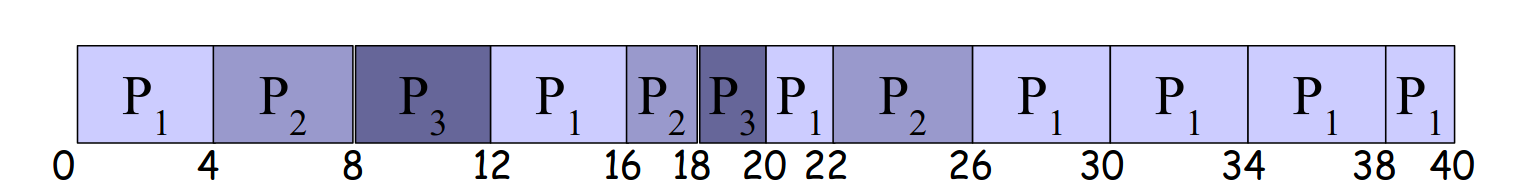
\includegraphics[width=0.5\linewidth]{Images/Screenshot 2024-12-23 at 15-06-19 so-02.1-scheduling - so-02.1-scheduling.pdf.png}
    \caption{}
\end{figure}

Tre processi: $P_1$, $P_2$, $P_3$
\newline
Lunghezza dei CPU-burst in ms ($P_1$: 10+14; $P_2$: 6+4; $P_3$: 6)
\newline
Lunghezza del quanto di tempo: 4
\newline
Tempo medio di turnaround (40+26+20)/3 = 28.66 ms
\newline
Tempo medio di attesa: (16+16+14)/3 = 15.33 ms
\newline
Tempo medio di risposta: 4 ms

\subsection{Scheduling a priorità}

Il round-robin fornisce le stesse possibilità di esecuzione a tutti i processi. 
Ma i processi non sono tutti uguali, infatti usando round-robin puro la visualizzazione dei un video MPEG potrebbe essere ritardata da un processo che sta per esempio smistando la posta, la lettera può aspettare mezzo secondo, il frame video no!

\textit{Vediamo quindi come impostare un round-robin con delle priorità...}

\paragraph{Descrizione:} a ogni processo è associata una specifica priorità, lo scheduler sceglie il processo pronto con priorità più alta.
\newline

Le priorità possono essere: 
\begin{itemize}
    \item \textbf{Definite dal sistema operativo:} vengono utilizzate una o più variabili per calcolare la priorità di un processo.
    \textit{Esempio: SJF è un sistema basato su priorità}
    \item \textbf{Definite esternamente:} le priorità non vengono definite dal sistema operativo, ma vengono imposte dal livello utente.
\end{itemize}

\begin{figure} [h]
    \centering
    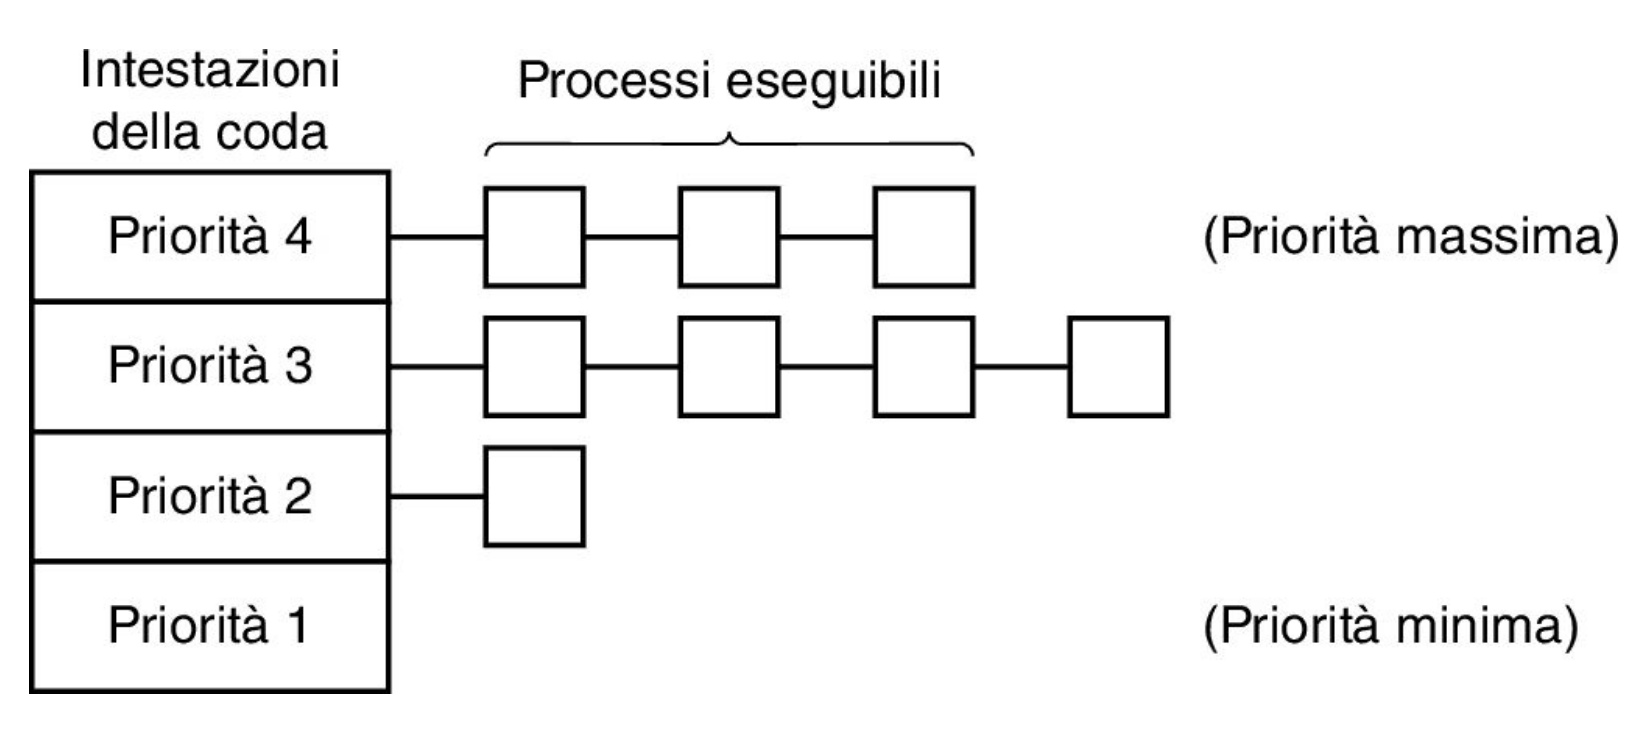
\includegraphics[width=0.6\linewidth]{Images/Screenshot 2024-12-23 at 17-14-31 so-02.1-scheduling - so-02.1-scheduling.pdf.png}
    \label{fig:enter-label}
\end{figure}

\subsubsection{Tecniche di assegnazione delle priorità}

\paragraph{Priorità statica:} la priorità non cambia durante la vita di un processo. Un problema di questa tecnica è che i processi a bassa priorità possono essere posti in starvation da processi ad alta priorità.

\paragraph{Priorità dinamica:} la priorità può variare durante la vita di un processo, è possibile utilizzare metodologie di priorità dinamica per evitare starvation

\paragraph{Priorità basata su aging:} tecnica che consiste nell'incrementare gradualmente la priorità dei processi
in attesa, posto che il range di variazione delle priorità sia limitato, nessun processo rimarrà in attesa per un tempo indefinito perché prima o poi raggiungerà la priorità massima.


\subsection{Scheduling a classi di priorità}

\paragraph{Descrizione:} è possibile creare diverse classi di processi con caratteristiche simili e assegnare ad ogni classe specifiche priorità. La coda ready viene quindi scomposta in molteplici "sottocode", una per ogni classe di processi.

\paragraph{Algoritmo:} uno scheduler a classi di priorità seleziona il processo da eseguire fra quelli pronti della classe a priorità massima che contiene processi.

\subsection{Scheduling multilivello}
\paragraph{Descrizione:} all'interno di ogni classe di processi, è possibile utilizzare una politica specifica adatta alle caratteristiche della classe. 

Uno scheduler multilivello cerca prima la classe di priorità massima che ha almeno un processo ready, sceglie poi il processo da porre in stato running coerentemente con la politica specifica della classe.
\newline

\textbf{Quattro classi di processi (priorità decrescente):}

\begin{itemize}
    \item processi server \textit{(priorità statica)}
    \item processi utente interattivi \textit{(round-robin)}
    \item altri processi utente \textit{(FIFO)}
    \item processo vuoto \textit{(FIFO banale)}
\end{itemize}

\section{Scheduling Real-Time}
In un sistema real-time la correttezza dell'esecuzione non dipende solamente dal valore del risultato, ma anche dall'istante temporale nel quale il risultato viene emesso.

\paragraph{Hard real-time:} le deadline di esecuzione dei programmi non devono essere superate in nessun caso.
\newline
\textit{Esempi: sistemi di controllo nei velivoli, centrali nucleari o per la cura intensiva dei malati...}

\paragraph{Soft real-time:} errori occasionali sono tollerabili.
\newline
\textit{Esempi: ricostruzione di segnali audio-video, transazioni interattive}
\newline

Esistono due tipi di processi RT (real-time).

\paragraph{Processi periodici:} sono periodici i processi che vengono riattivati con una cadenza regolare (periodo).
\newline
\textit{Esempi: controllo assetto dei velivoli, basato su rilevazione periodica dei parametri di volo.}

\paragraph{Processi aperiodici:} i processi che vengono scatenati da un evento sporadico.
\newline
\textit{Esempio: l'allarme di un rilevatore di pericolo}

\newpage
\subsection{Esempi di Scheduler RT}
\subsubsection{Rate Monotonic}
\paragraph{Descrizione:} è una politica di scheduling, dove ogni processo periodico deve completarsi entro il suo periodo, tutti i processi sono indipendenti e la preemption avviene istantaneamente e senza overhead.

Viene assegnata staticamente una priorità a ogni processo, processi con frequenza più alta \textit{(i.e. periodo più corto)} hanno priorità più alta. Ad ogni istante, viene eseguito il processo con priorità più alta (facendo preemption se necessario).

\subsubsection{Earliest Deadline First (EDF)}
\paragraph{Descrizione:} è una politica di scheduling per processi periodici real-time, viene scelto di volta in volta il processo che ha la deadline più prossima. 

Viene detto "a priorità dinamica" perchè la priorità relativa di due processi varia in momenti diversi.

